% !TEX root = ../main.tex
\chapter{Introduction}
\section{Machine Learning}
Machine Learning based technologies solve specific tasks very well, while AI chatbots have quite broad and general capabilities.
However classic machine learning predictions may not be sufficient for decision-making. 
Machine learning requires a 'supervisor' that provides meaningful data of the phenomenon we want to characterize. Typically we need $(x, y)$ and we look for a relationship $F$.
In many scenarios this is not feasible. 

RL aims to solve cases where data must be collected 'in the wild' (agent interacts with the world and learns how to maximize some objectives).

\section{Limits of Supervised Learning}
There are some limits for supervised learning techniques like RL:
\begin{itemize}
    \item Data are not aviable without interacting with the world;
    \item Collected data may not be explicitly associated to an action;
    \item Time matters: we don't always have i.i.d. data;
    \item In many settings, supervised learning do not envision long-term scenarios.
\end{itemize}

\section{RL Formalism}
\begin{itemize}
    \item An \textbf{agent}: entity aiming at solving the task;
    \item A set of \textbf{states ($\textit{S}$)} in which the agent can be;
    \item A set of \textbf{actions $(\textit{A})$} that can be taken by the agent;
    \item An \textbf{environment} with which the agents interacts, and that changes after the agent takes an action (also provides back a \textbf{reward $(\textit{R})$});
    \item The agent can be more interested in long-term rewards more than short-term.
\end{itemize}

\begin{figure}[htbp]
    \centering
    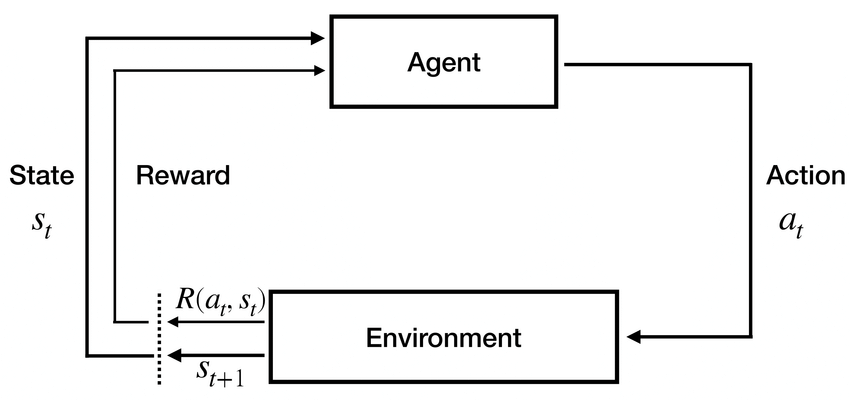
\includegraphics[width=0.7\textwidth]{./figures/chapter1/Reinforcement-Learning-framework-adapted-from-Sutton-and-Barto-2018-1915045654.png} 
    \caption{Markov Decision Process scheme.}
    \label{fig:MDP}
\end{figure}

\section{RL Problem}
The agent could initially know very little about the environment and about which reward and next states a give action from a given state could lead to. In other terms the dynamics of the environment is not known in advance, they must be learned by interaction with the environment.
The goal of the agent is to maximize long term rewards. 